% Author: Rasmus Pank Roulund
% Inspired by figure in:
% Howells, Peter og Bain, Keith (2007). Financial markets and
% institutions. 5. udg. Essex: Pearson Education.
\documentclass{minimal}
\usepackage{tikz}
\usetikzlibrary{arrows,positioning} 
\tikzset{
    %Define standard arrow tip
    >=stealth',
    %Define style for boxes
    punkt/.style={
           rectangle,
           shade,
           top color = blue,
           bottom color = white,
           rounded corners,
           draw=blue!40!black!60, very thick,
           text width=5cm,
           minimum height=2em,
           text centered},
    % Define arrow style
    pil/.style={
           ->,
           thick,
           shorten <=2pt,
           shorten >=2pt,}
}

\begin{document}

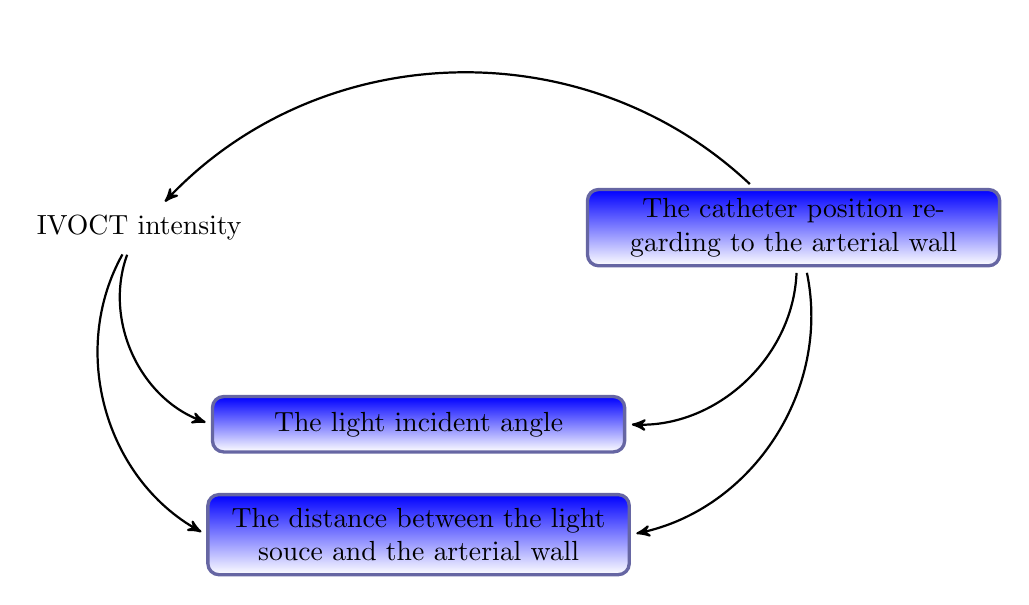
\begin{tikzpicture}[node distance=2cm, auto,]
 %nodes
 \node[punkt] (market) {The light incident angle};
 \node[punkt, inner sep=5pt,below=0.5cm of market]
 (formidler) {The distance between the light souce and the arterial wall};
 % We make a dummy figure to make everything look nice.
 \node[above=of market] (dummy) {};
 \node[punkt, right=of dummy] (t) {The catheter position regarding to the arterial wall}
   edge[pil,bend left=45] (market.east) % edges are used to connect two nodes
   edge[pil, bend left=45] (formidler.east); % .east since we want
                                             % consistent style
 \node[left=of dummy] (g) {IVOCT intensity}
   edge[pil, bend right=45] (market.west)
   edge[pil, bend right=45] (formidler.west)
   edge[pil,<-, bend left=45] node[auto] {} (t);
\end{tikzpicture}

%\vspace{1em}
%\emph{Inspired by figure 1.1 in ``Financial Markets and Institutions'' 5E
%  by Howells and Bain.}
\end{document}

%%% Local Variables:
%%% mode: latex
%%% TeX-master: t
%%% End: